\indent En lo que sigue, mostraremos buenos y malos casos para nuestro algoritmo, y a su vez, daremos el tiempo estimado 
seg\'un la complejidad del algoritmo calculada anteriormente.\\


A continuaci\'on mostraremos un gr\'afico de tiempos comparativo entre distintas familias de casos:\\ 

\vspace*{0.3cm} \vspace*{0.3cm}
  \begin{center}
% 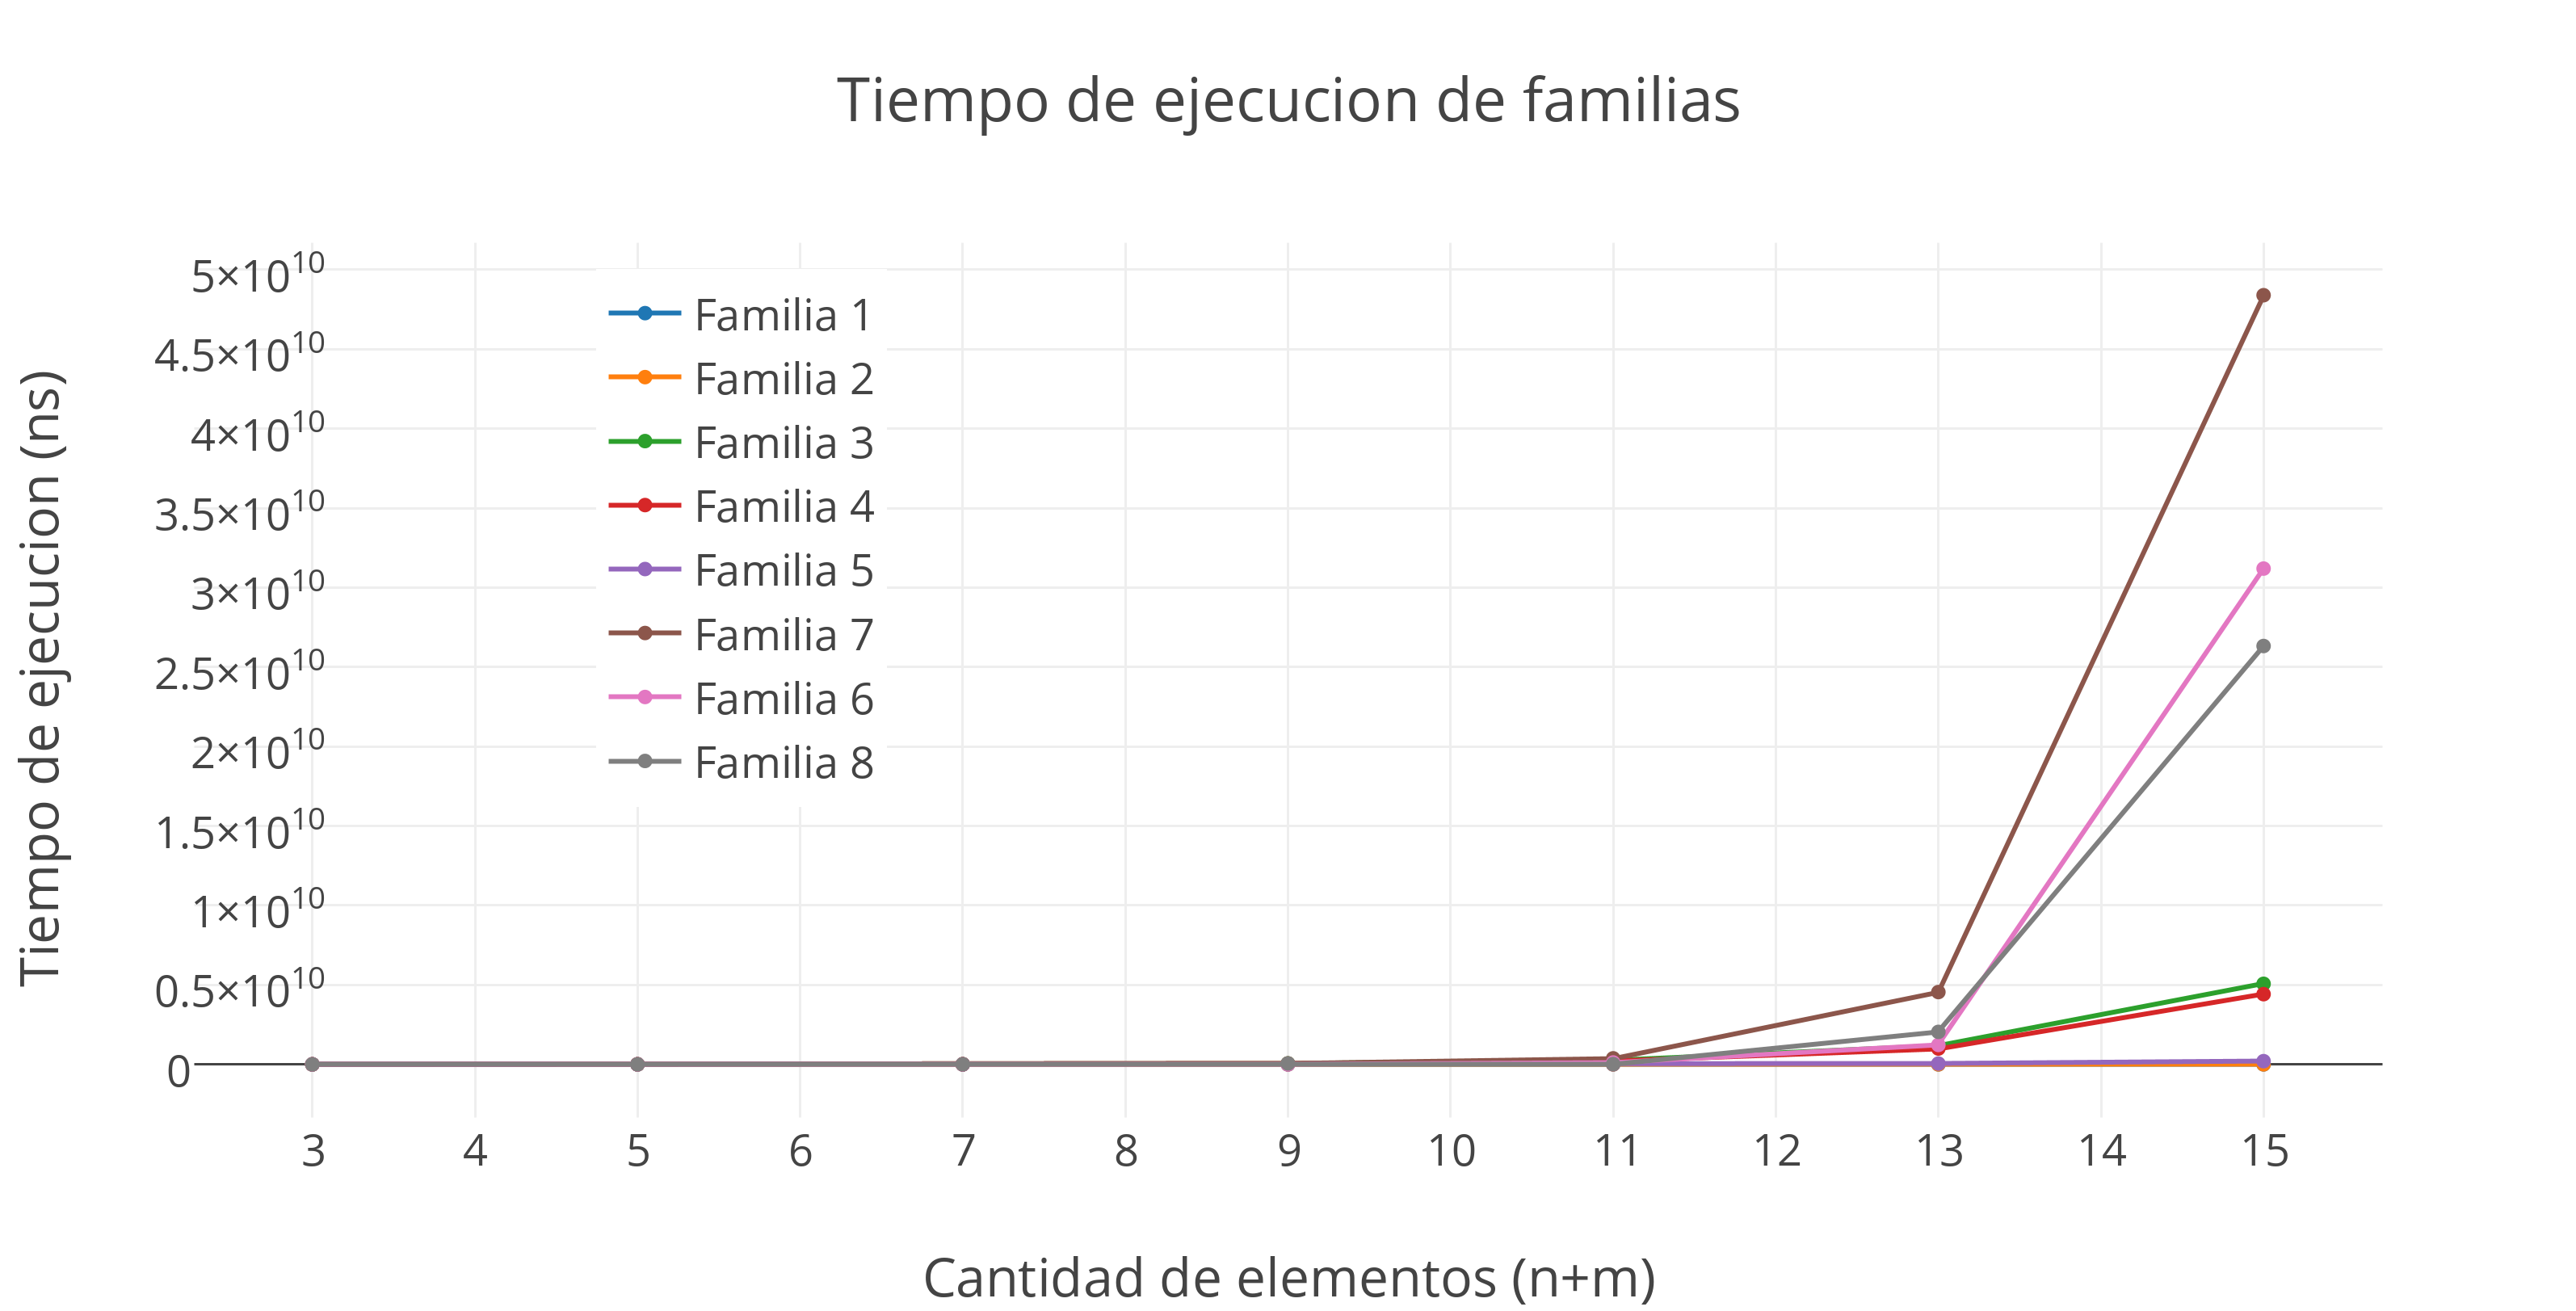
\includegraphics[scale=0.4]{./EJ1/comparativo.png}
 {            $Gr$\'a$fico$ \ 1.1 - $Comparativo$}
  \end{center}
  \vspace*{0.3cm}
  
Se puede observar en el gr\'afico, tres funciones las cuales representan el tiempo de ejecuci\'on de las familias de casos:\\
\begin{itemize}
\item Sin soluci\'on o con camino m\'inimo inmediato
\item Rompiendo una cantidad de P-1 paredes
\item M\'ultiples caminos a destino posibles
\end{itemize}


Como se observa en el gr\'afico la funci\'on representativa de la flia n\'umero 1, presenta una mejor performance en relaci\'on a las otras. Esto se debe a que en el primer paso no puede salir por ning\'un camino posible, o su adyacente es el nodo destino por lo tanto chequea solo los nodos adyacentes del origen y finaliza su ejecuci\'on.

Por lo cual, el mejor caso teniendo en cuenta a nivel performance de nuestro algoritmo ser\'a cuando se presente un problema \textbf{Sin soluci\'on o con camino m\'inimo inmediato}

Los grafos que representan lo dicho ser\'ian los siguiente:\\

\vspace*{0.3cm} \vspace*{0.3cm}
  \begin{center}
%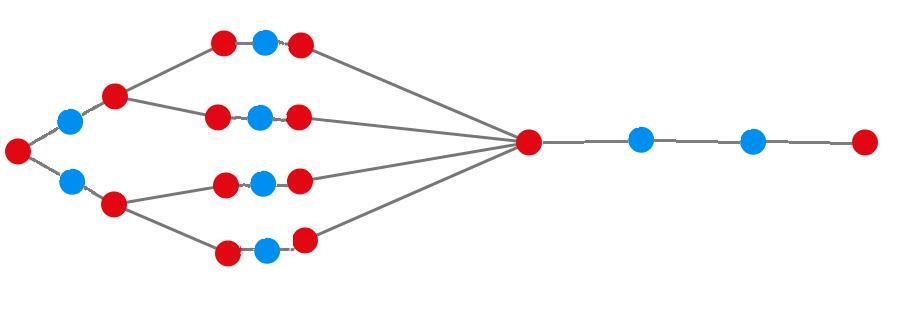
\includegraphics[scale=0.65]{./EJ1/ej1grafomejorcaso.jpeg}
{$Ejemplo Grafo$ \ G1.1 - $Mejor$ $Caso$ $Con$ $P=0$ }
  \end{center}
  \vspace*{0.3cm}

\vspace*{0.3cm} \vspace*{0.3cm}
  \begin{center}
%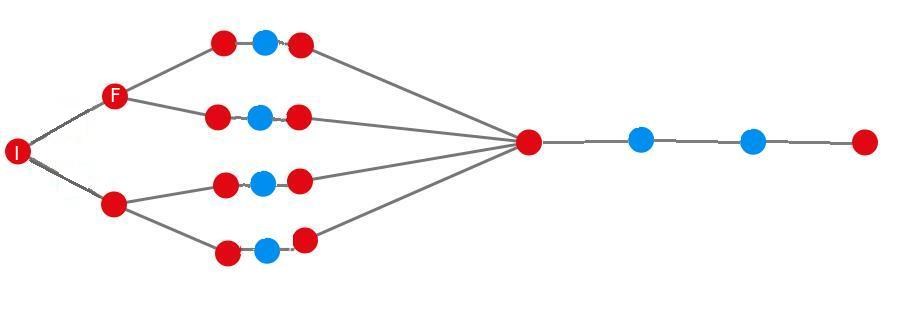
\includegraphics[scale=0.65]{./EJ1/ej1grafomejorcaso2.jpeg}
{$Ejemplo Grafo$ \ G1.1 - $Mejor$ $Caso$ $Con$ $P=0$ }
  \end{center}
  \vspace*{0.3cm}

Para una mayor observaci\'on desarrollamos el siguiente gr\'afico con las instancias:\\

\vspace*{0.3cm} \vspace*{0.3cm}
  \begin{center}
 %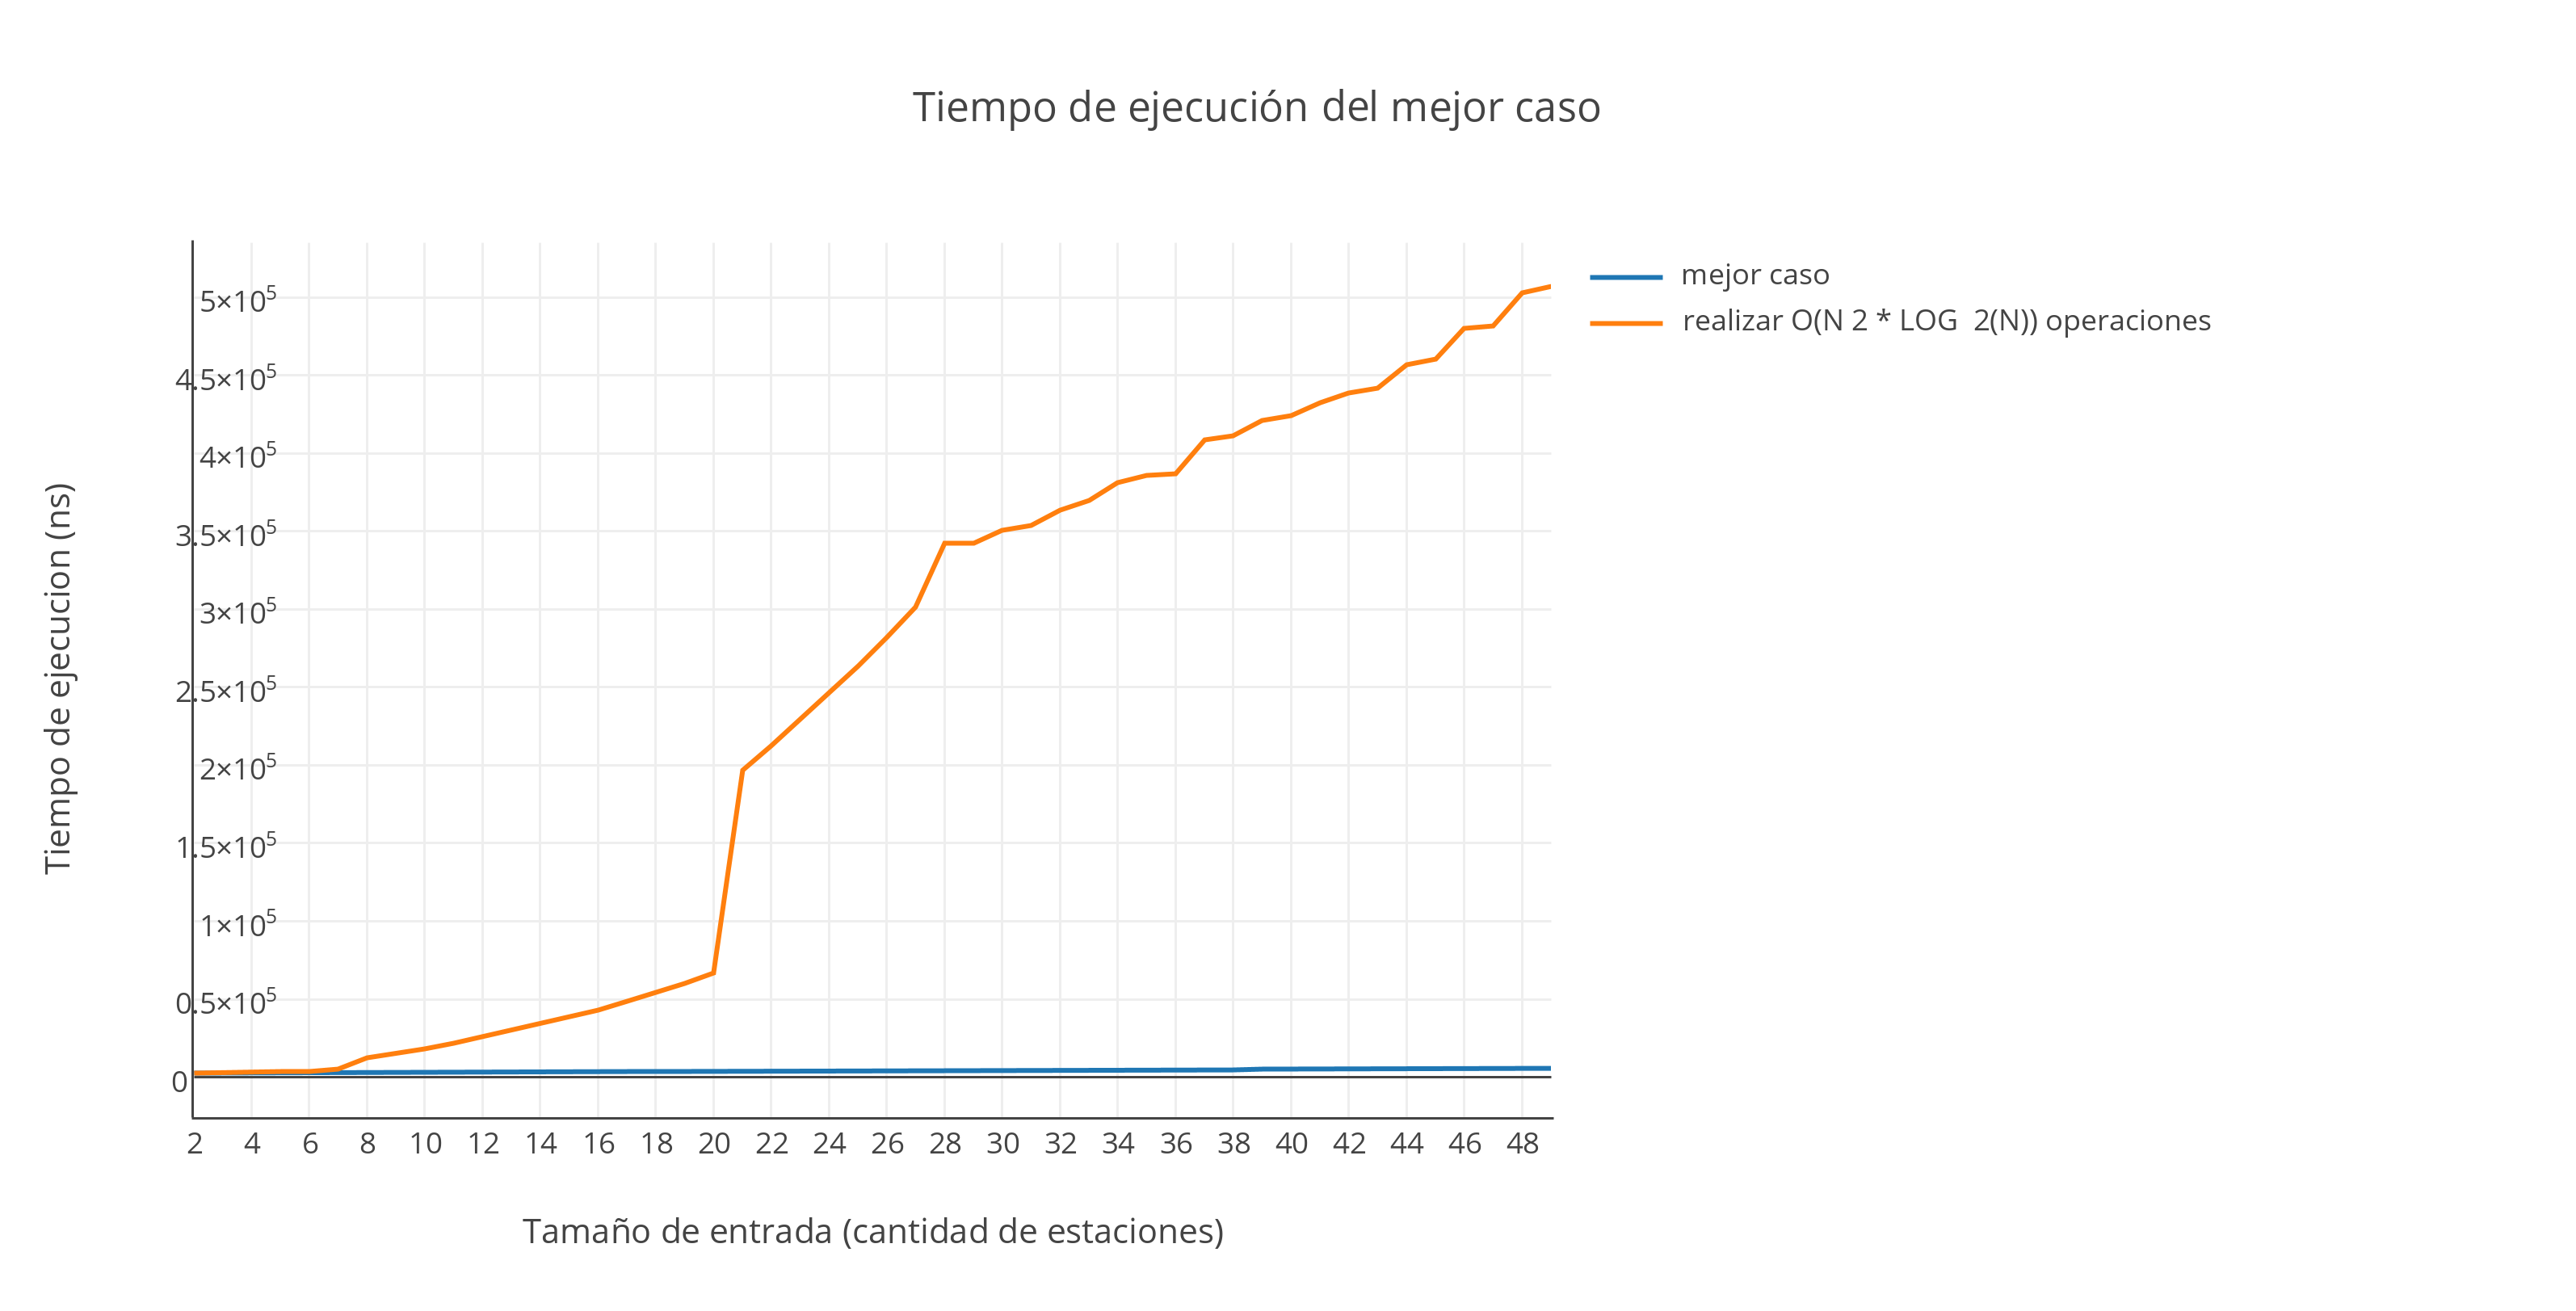
\includegraphics[scale=0.65]{./EJ1/mejorcaso.png}
 {$Gr$\'a$fico$ \ 1.1 - $Mejor$ $Caso$}
  \end{center}
  \vspace*{0.3cm}

Como la complejidad que calculamos se basa en la cantidad de nodos posibles que puede haber multiplicado por las paredes contrastaremos nuestras mediciones con los valores de O(F $\times$ C $\times$ P).\\

Luego, dividiendo la funci\'on resultante de nuestro algoritmo sobre el tiempo que demanda realizar O(F $\times$ C $\times$ P) nos da lo siguiente:

\vspace*{0.3cm} \vspace*{0.3cm}
  \begin{center}
 %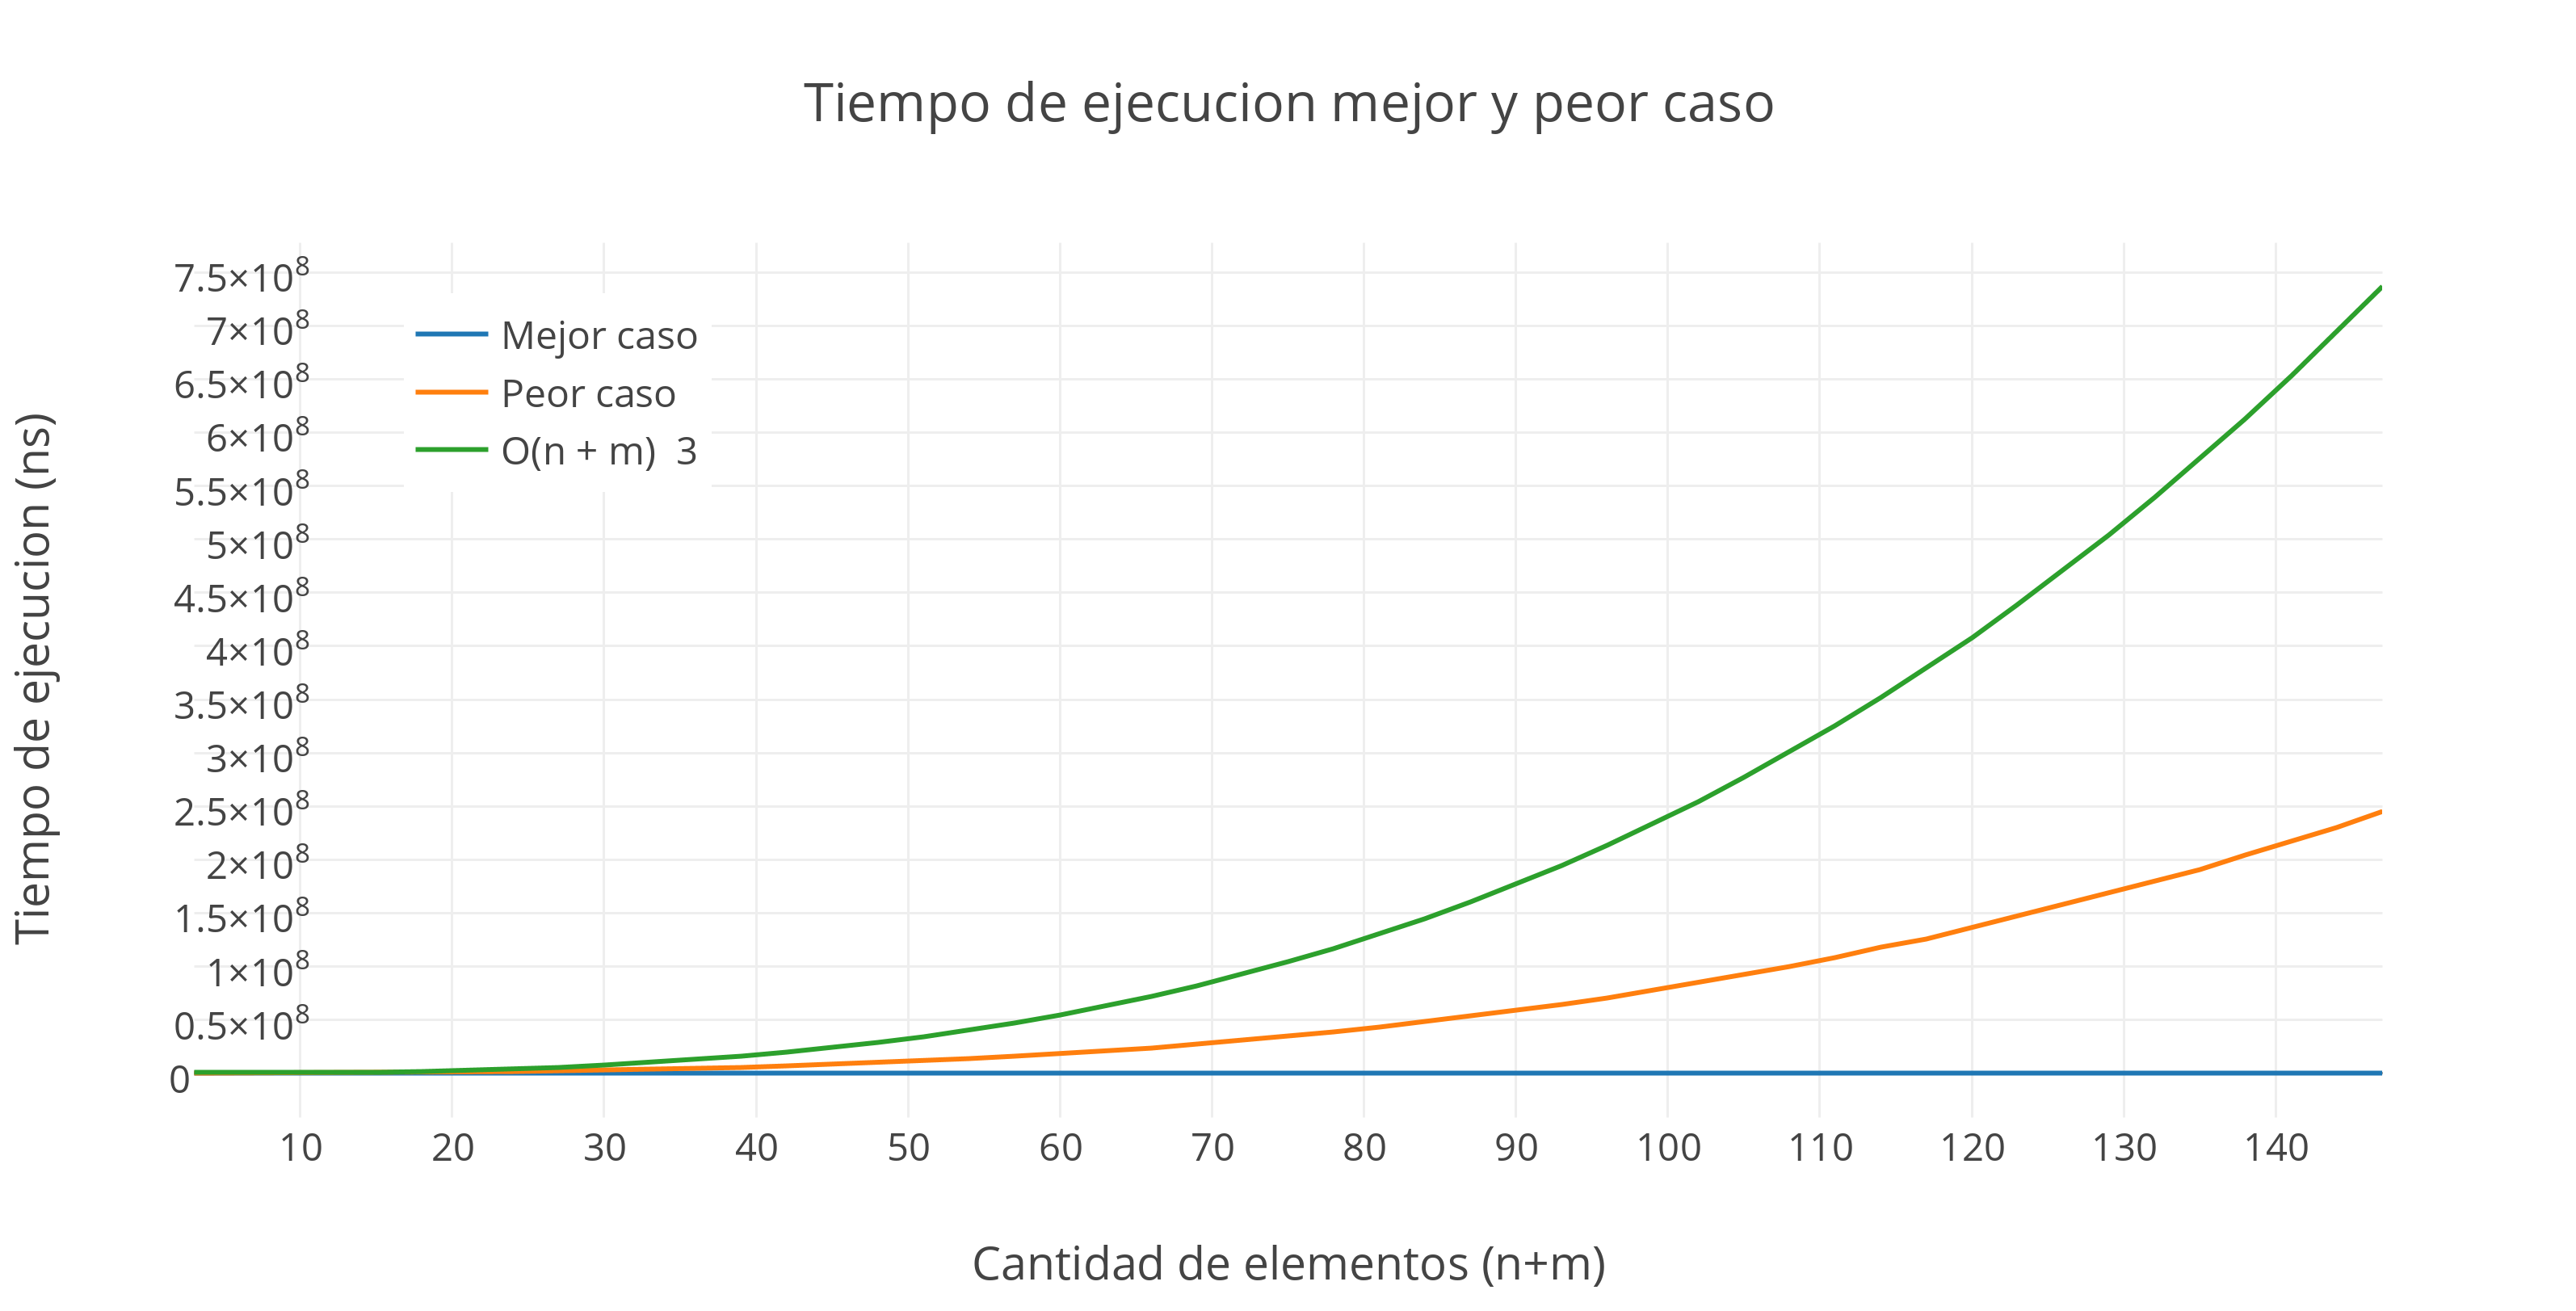
\includegraphics[scale=0.65]{./EJ1/mejorcaso1.png}
 {$Gr$\'a$fico$ \ 1.2 - $Mejor$ $Caso$ $Sobre$ $Complejidad$ $O(F \times C \times P)$}
  \end{center}
  \vspace*{0.3cm}

 Para obtener dichas instancias nos resulto prudente realizar aproximadamente unas 20 corridas con el mismo input y sacar el promedio de estas 20 corridas para cada instancia para obtener resultados m\'as consisos.\\ 

Se observa en el gr\'afico 1.1 como la funci\'on que representa al tiempo de nuestro algoritmo en el mejor caso es considerablemente mejor que la funci\'on de la cota te\'orica, mientras que al realizar la divisi\'on entre ambas funciones se llega a que la misma nunca supera el valor 0.9 quedando siempre por debajo de 1 mostrando as\'i que para cualquier valor de entrada posible el mejor caso queda siempre en el orden de  O(F $\times$ C $\times$ P).\\

Luego, uno de los peores casos para nuestro algoritmo es en el cual  \textbf{se debe recorrer todos los posibles caminos ya que son todos exactamente iguales}, esto se da as\'i ya que nuestro algoritmo chequea todos los caminos posibles y como todos pueden ser soluci\'on posible avanza por todos y llega al final del laberinto con el mismo valor en todos los posibles caminos\\

\vspace*{0.3cm} \vspace*{0.3cm}
  \begin{center}
%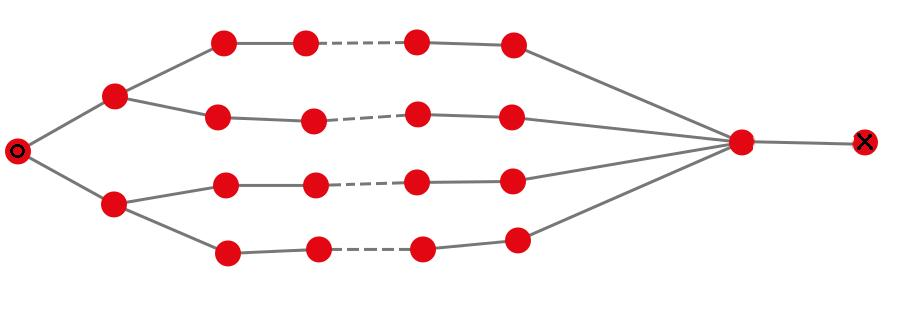
\includegraphics[scale=0.65]{./EJ1/ej1grafopeorcaso.jpeg}
{$Ejemplo Grafo$ \ G1.2 - $Peor$ $Caso$}
  \end{center}
  \vspace*{0.3cm}

Para este grafo realizamos las respectivas mediciones las cuales arrojaron los siguientes resultados:\\


\vspace*{0.3cm} \vspace*{0.3cm}
  \begin{center}
%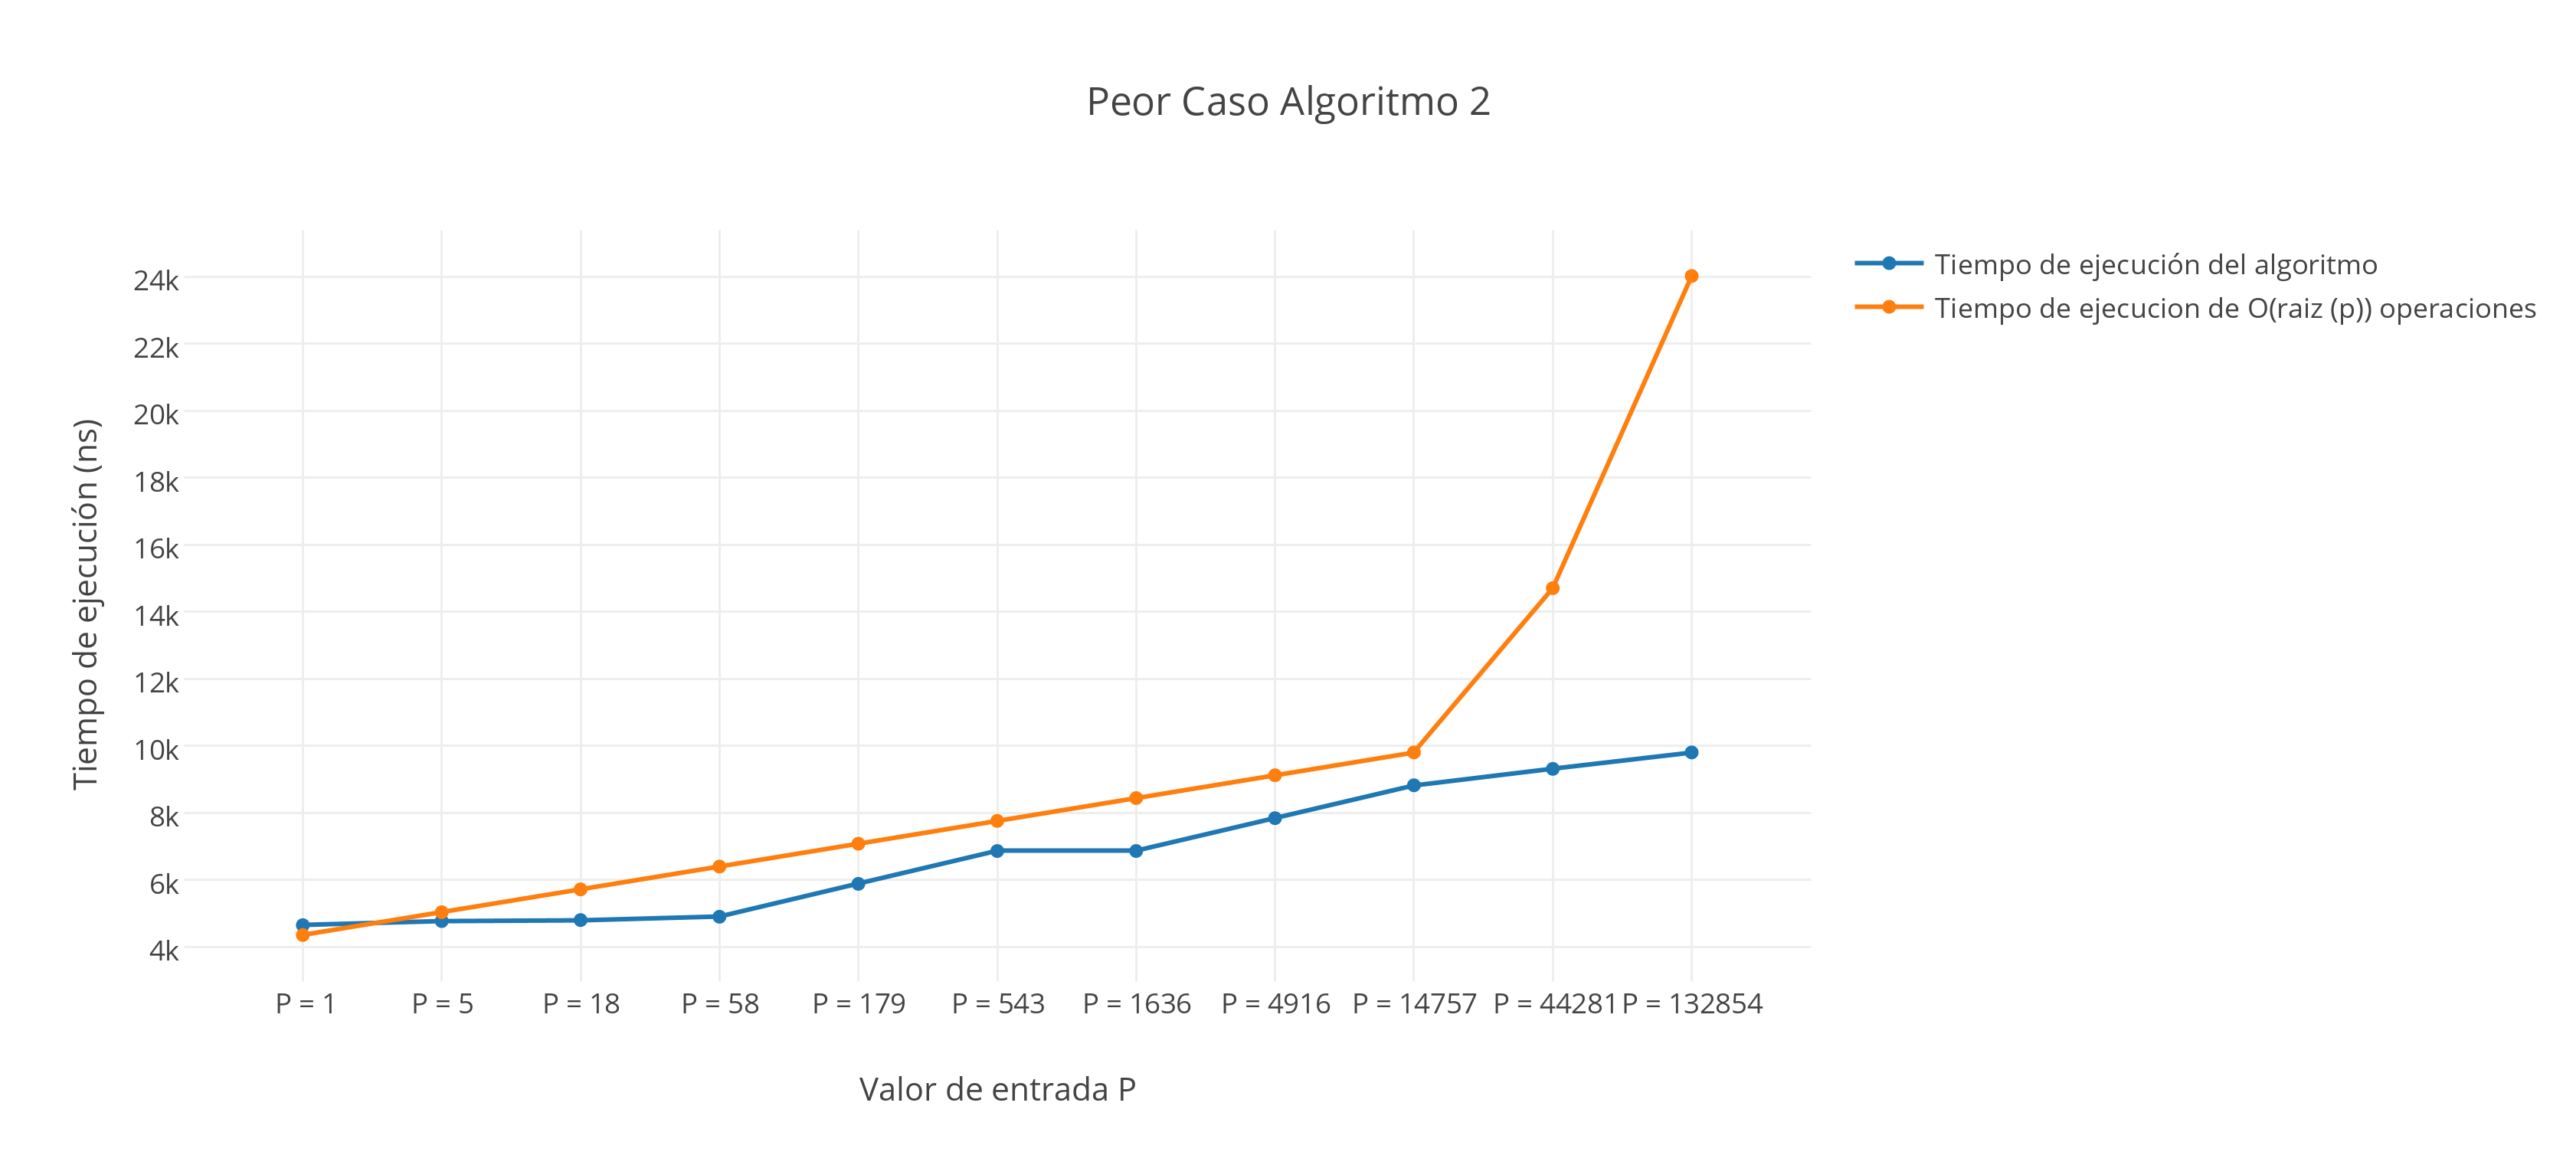
\includegraphics[scale=0.4]{./EJ1/peorcaso.png}
{$Gr$\'a$fico$ \ 1.3 - $Peor$ $Caso$}
  \end{center}
  \vspace*{0.3cm}

Dividiendo por la complejidad se llego a lo siguiente:\\

\vspace*{0.3cm} \vspace*{0.3cm}
  \begin{center}
%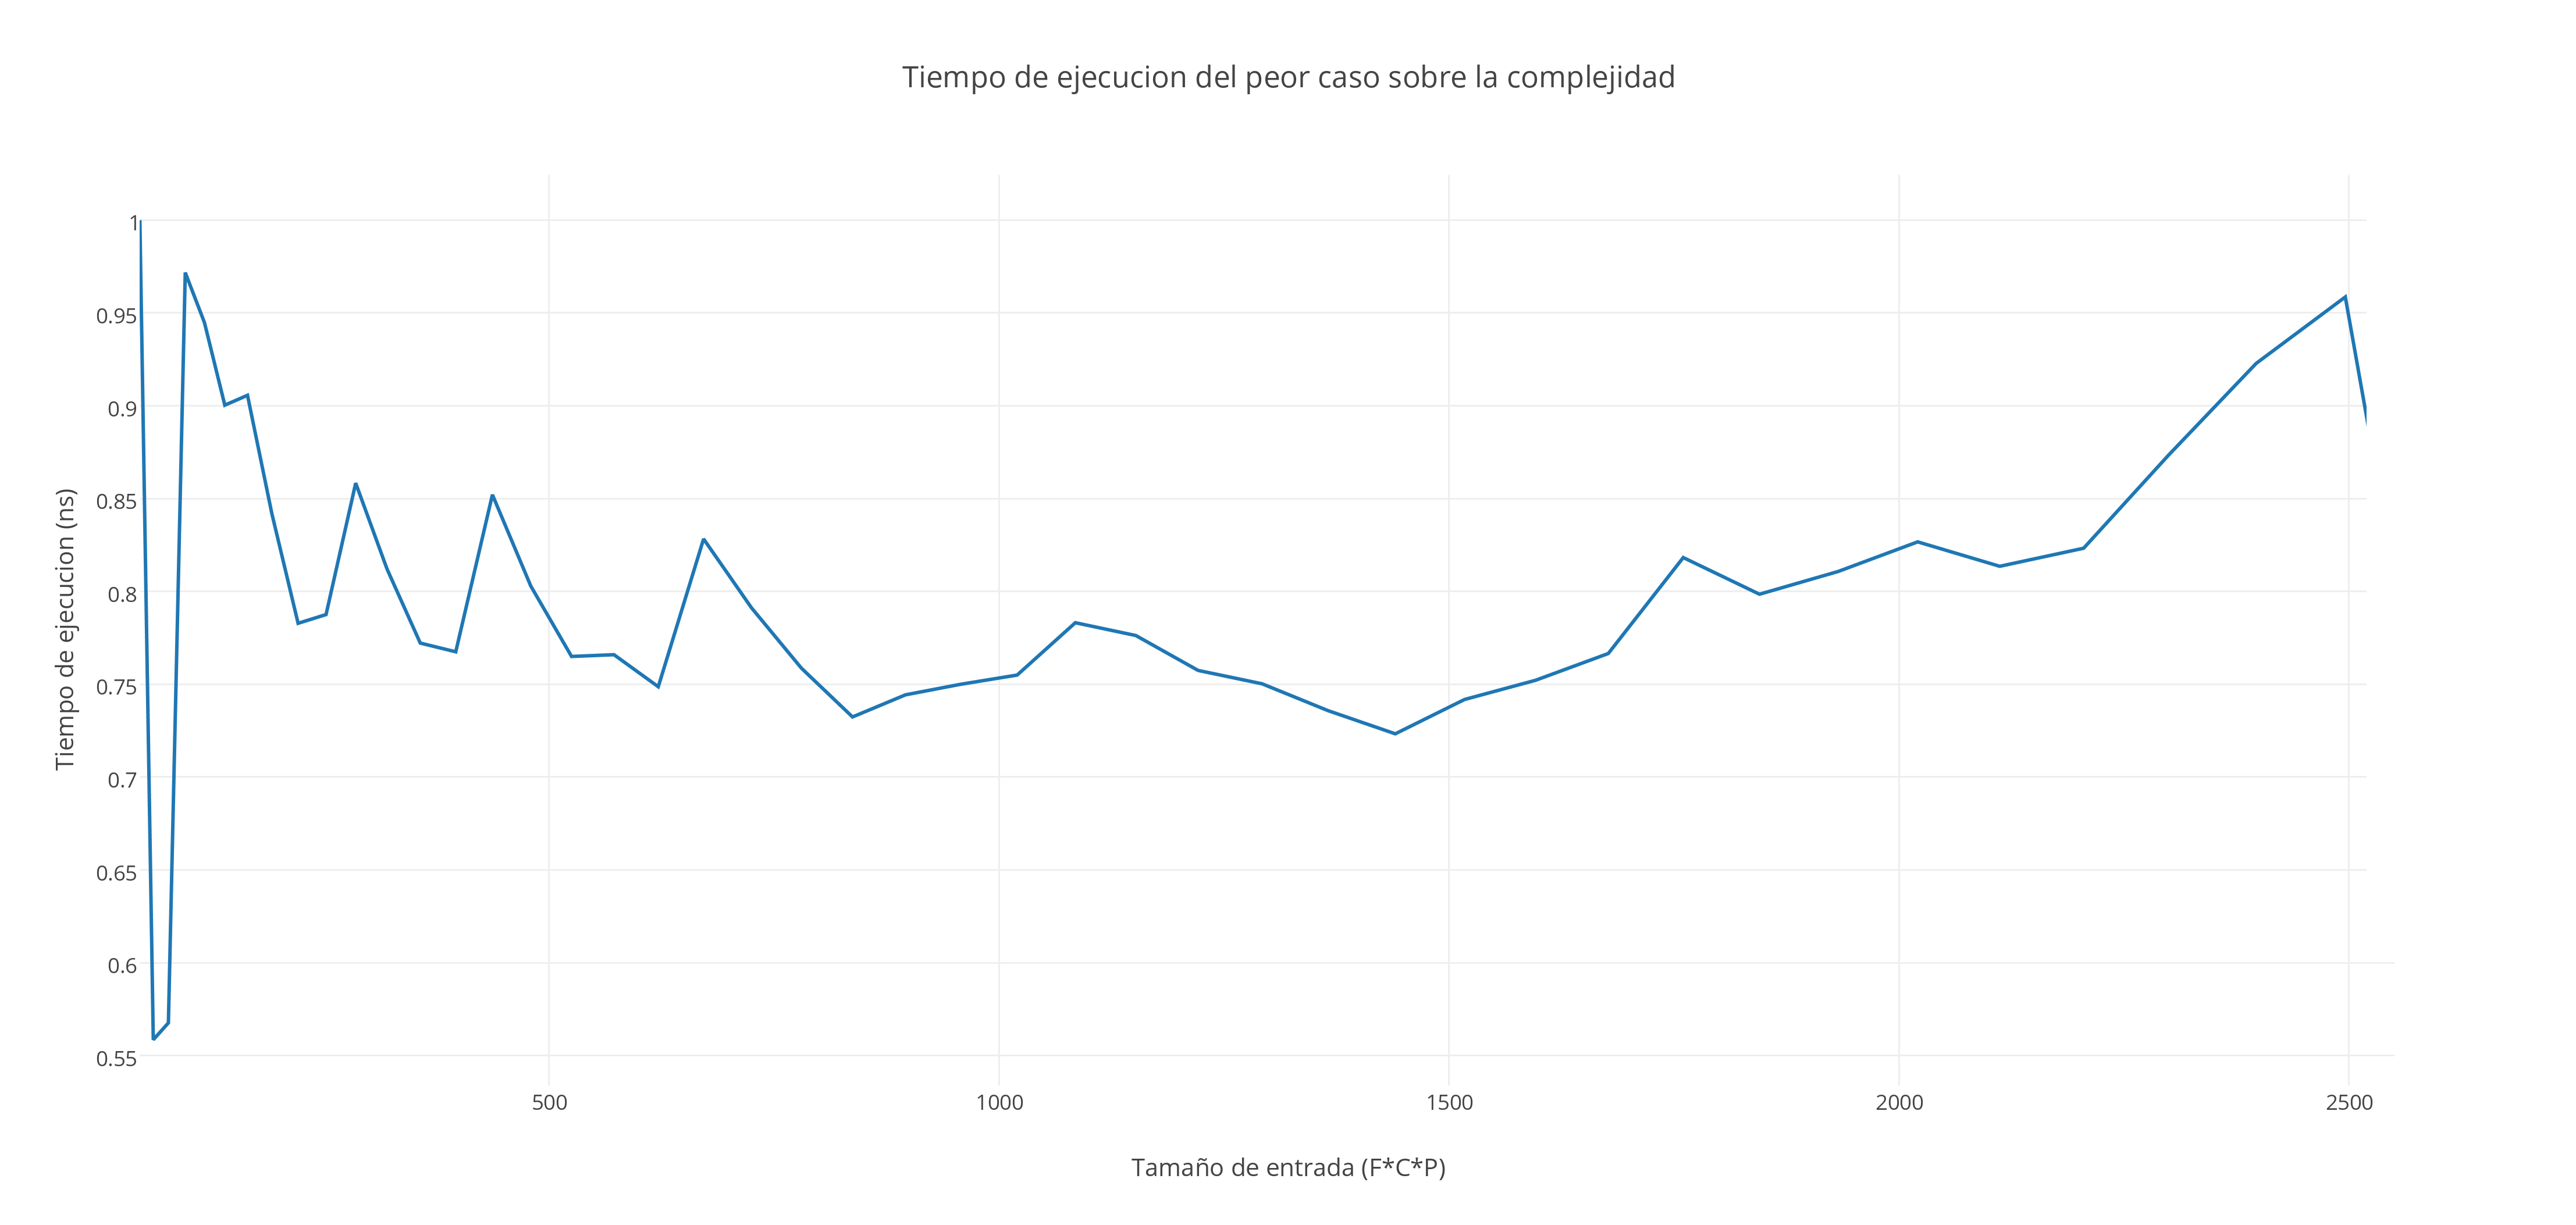
\includegraphics[scale=0.5]{./EJ1/peorcaso1.png}
{$Gr$\'a$fico$ \ 1.4 - $Peor$ $Caso$ $Sobre$ $Complejidad$ $O(F \times C \times P)$}
  \end{center}
  \vspace*{0.3cm}

 Para obtener dichas instancias nos resulto prudente realizar aproximadamente unas 20 corridas con el mismo input y sacar el promedio de estas 20 corridas para cada instancia para obtener resultados m\'as consisos.\\ 

Podemos observar en la figura 1.3 como la funci\'on resultante de nuestro algoritmo en el peor caso se mantiene por debajo de la funci\'on final del tiempo de realizar O(F $\times$ C $\times$ P) operaciones lo cual fue la complejidad precalculada. Y, en el gr\'afico 1.4 es posible observar como la funci\'on obtenida presenta disversos picos los cuales nunca llegan a superar 1, y cuando el tamaño de entrada aumenta la funci\'on queda asintotizada por 0.95.\\

Por \'ultimo mostraremos un gr\'afico comparativo con el mejor, el peor y el caso promedio contra la complejidad precalculada .\\

  
  \vspace*{0.3cm} \vspace*{0.3cm}
  \begin{center}
%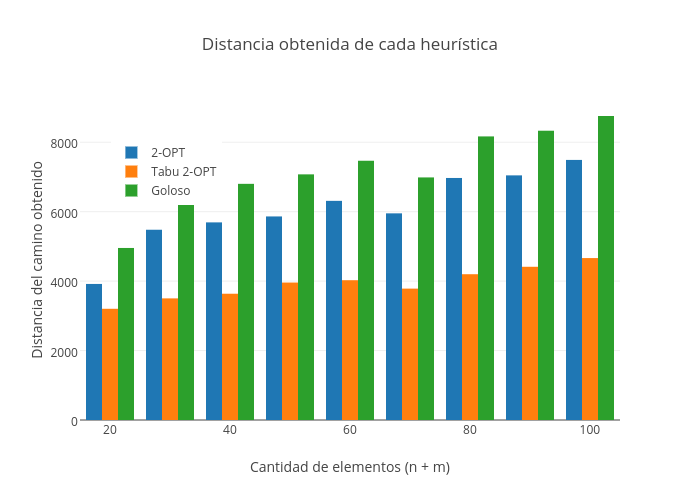
\includegraphics[scale=0.4]{./EJ1/comparativo1.png}
{$Gr$\'a$fico$ \ 1.5 - $Comparativo$}
  \end{center}
  \vspace*{0.3cm}
  
 Es visible en este gr\'afico comparativo como las funciones relacionadas a nuestro algoritmo estan acotadas por la funci\'on de la complejidad te\'orica.

Mostraremos a continuaci\'on un caso en el cual se dejaron fijas las variables F y C, ambas en 50 y se trabajo con P movil para ver como se comporta nuestro algoritmo en esta situaci\'on.

\vspace*{0.3cm} \vspace*{0.3cm}
  \begin{center}
%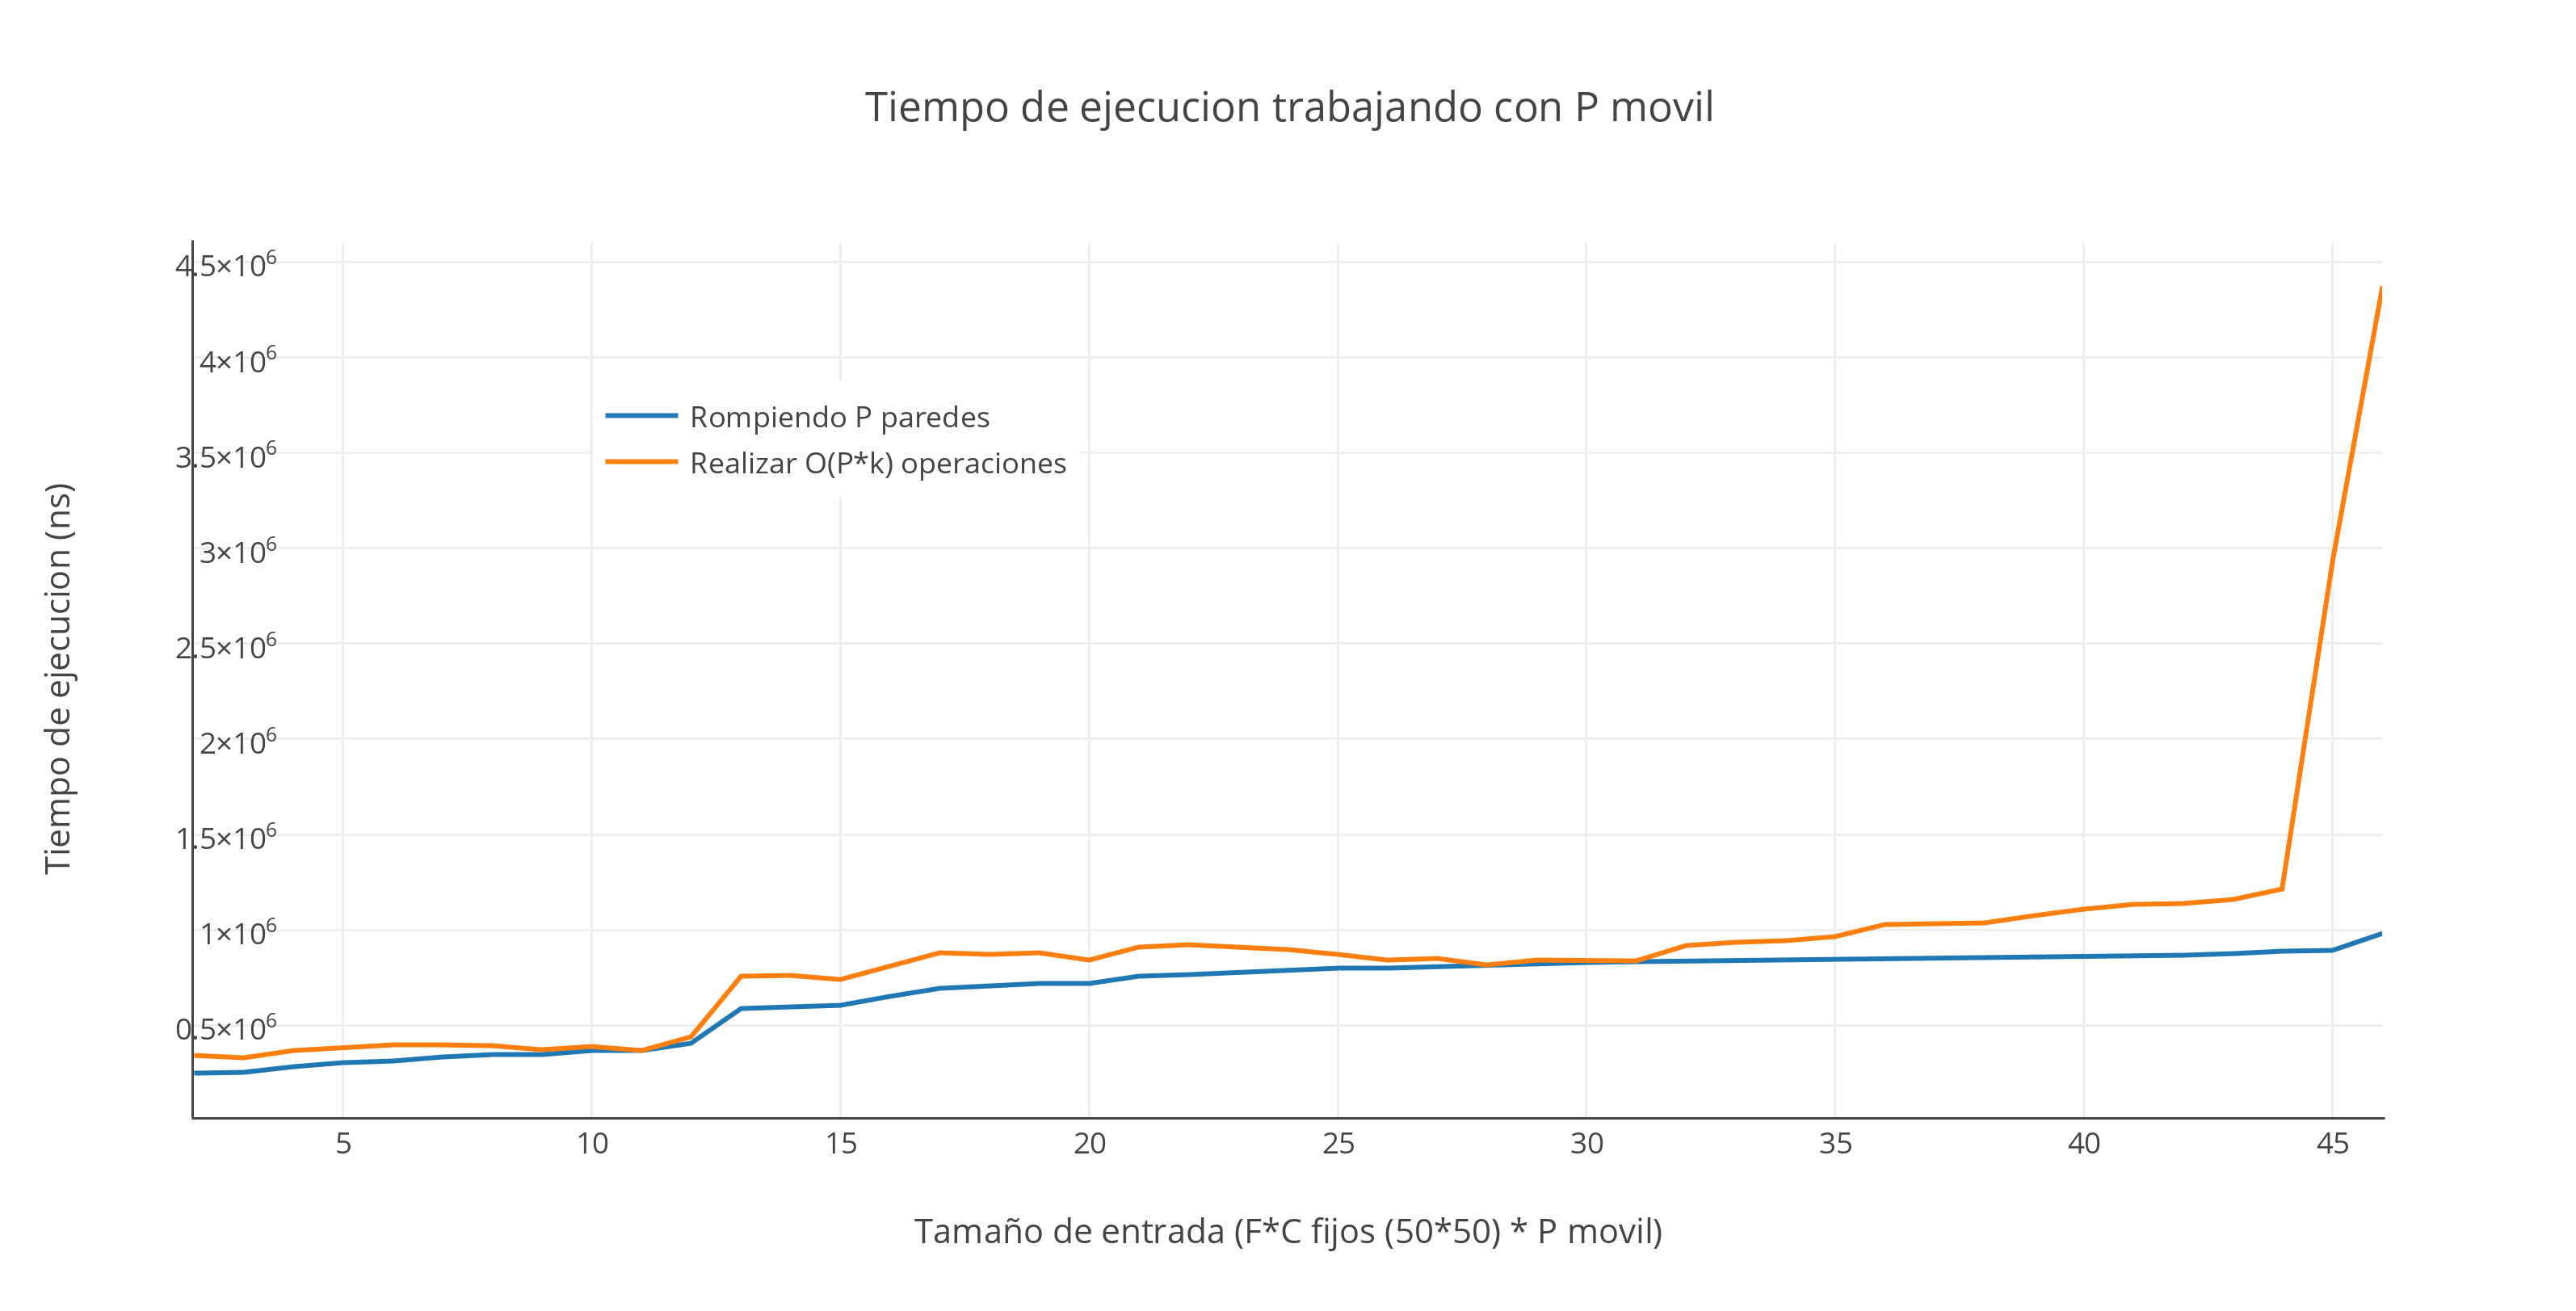
\includegraphics[scale=0.65]{./EJ1/pMovil.png}
{$Gr$\'a$fico$ \ 1.6 - $P$ $movil$ $y$ $F,C$ $Fijos$}
  \end{center}
  \vspace*{0.3cm}

Se puede observar en el gr\'afico 1.6 como al trabajar con este caso en el cual a medida que P aumenta es necesario romper P paredes para llegar a destino, la funci\'on resultante se comporta de la misma manera que O(P), chequeando de esta forma que trabajando con una cantidad fija de nodos nuestro algoritmo realiza O(P) operaciones por cada elemento del grafo.\\

Luego de lo mostrado, se pudo observar que, tanto en el mejor como en el peor caso nuestro algoritmo se encuentra en el orden de la complejidad calculada.